\chapter{Tube notching basics}

Tube Notching is a useful machining process in applications ranging from HVAC to metal framing. In these applications, it is common for low-gauge hollow tubing to be notched prior to welding or fastening. Notching is a process involving the removal of a section or end of a metal or plastic tube such that they can be coped with one another. 

Notches vary greatly depending on their application. The following figures are examples of welded round tubes:
% pictures! car frames, guide rails, etc
\begin{figure}[htp]
    \centering
    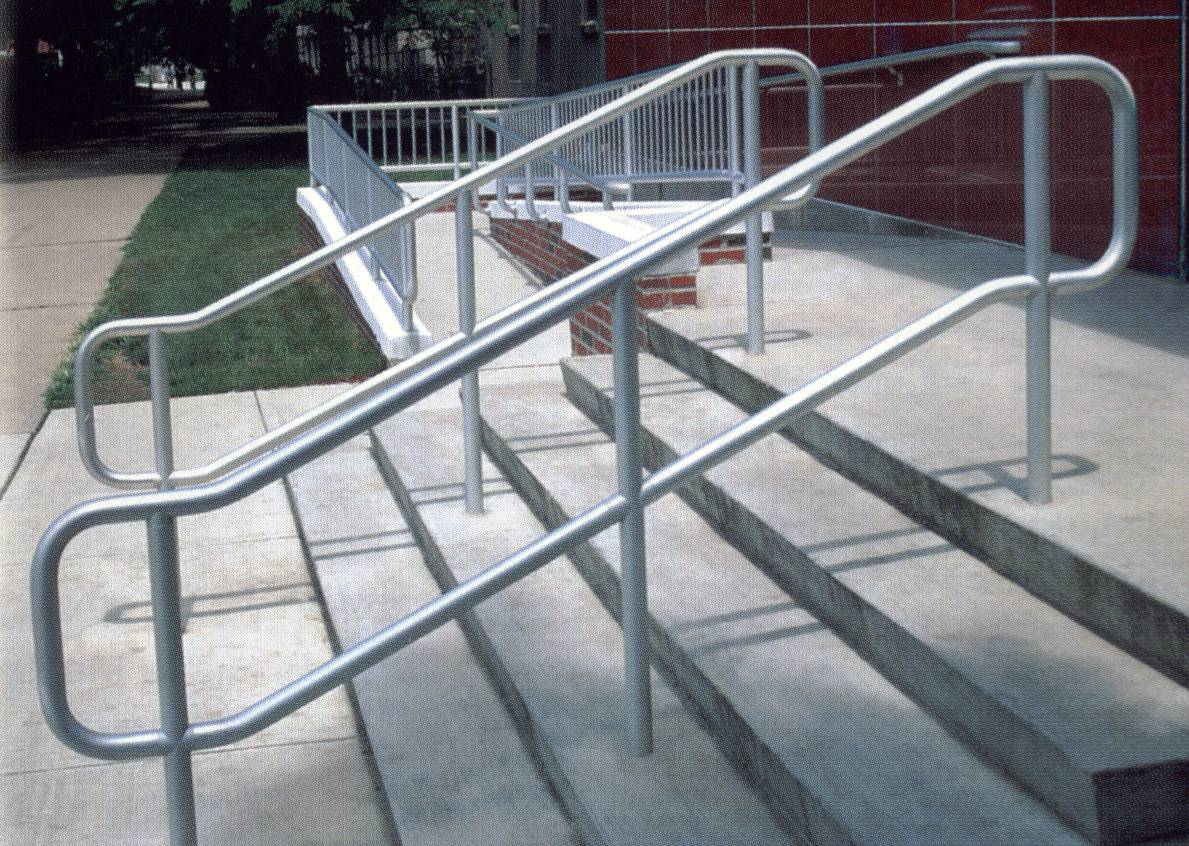
\includegraphics[width=0.4\textwidth]{./images/Chapter1-Basics/Railing}
    \caption{Hand rail for stairs}
    \label{fig:Stairs}
\end{figure}
\begin{figure}[htp]
    \centering
    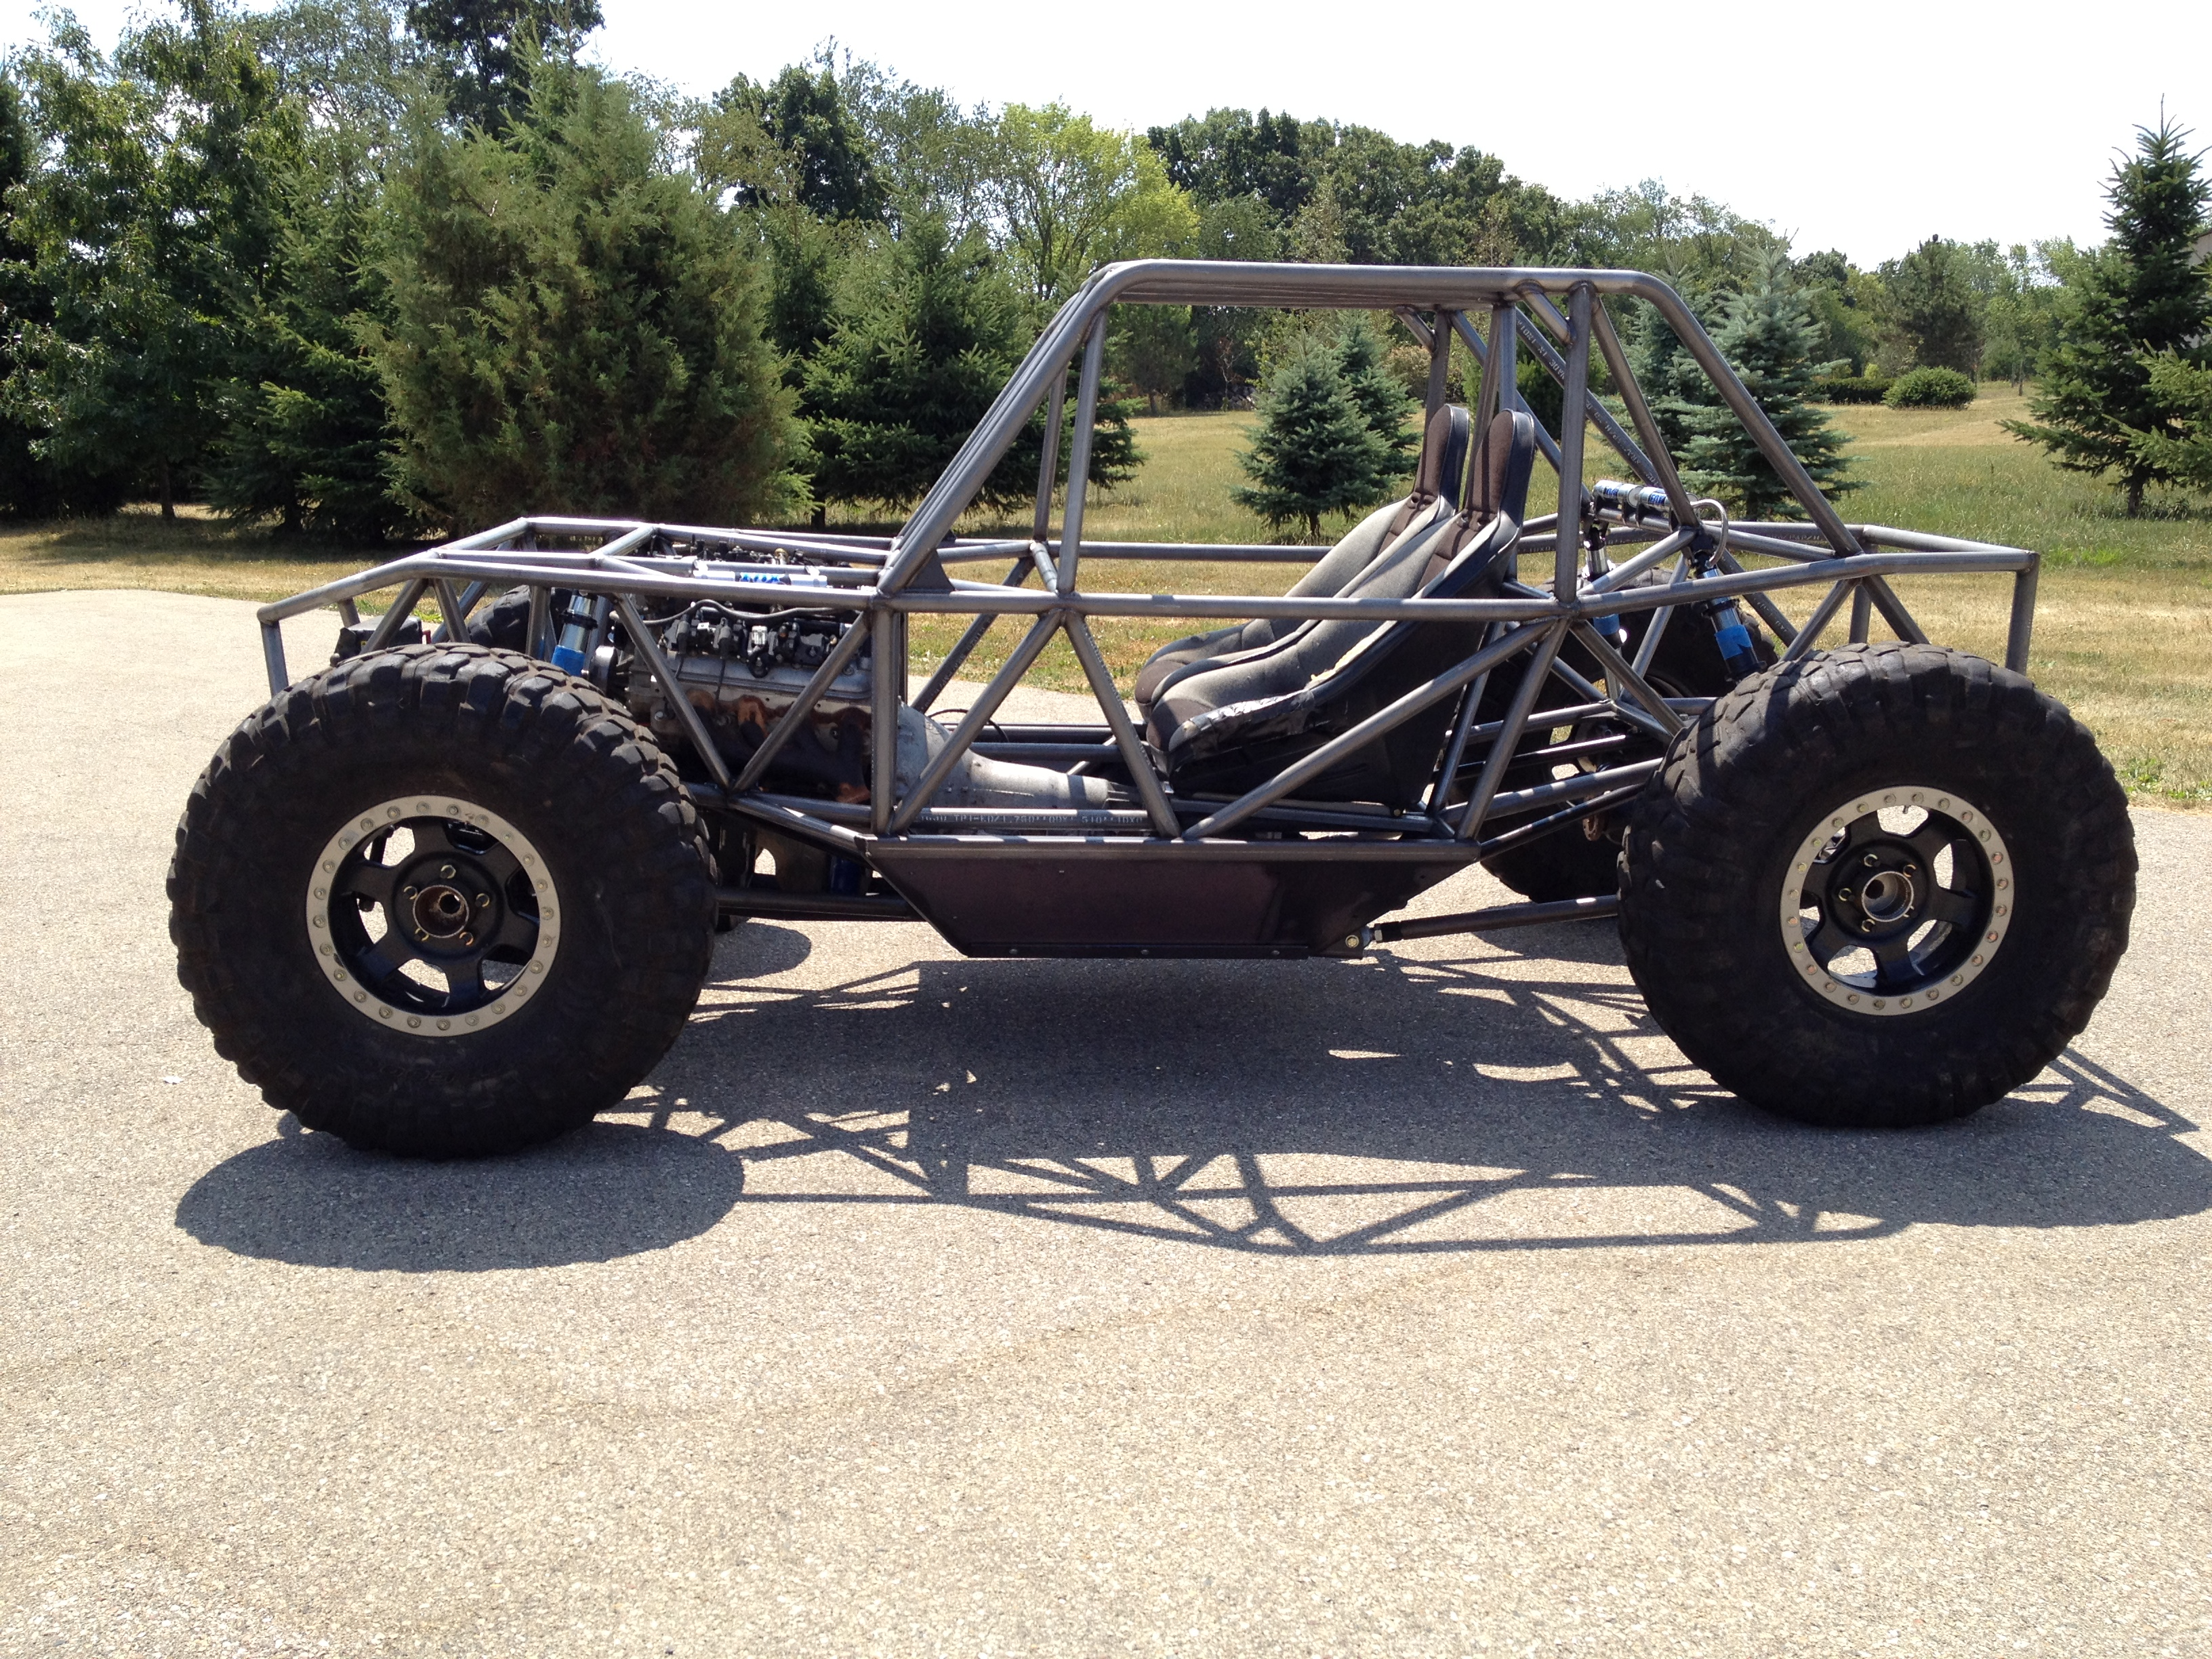
\includegraphics[width=0.4\textwidth]{./images/Chapter1-Basics/Rock Buggy}
    \caption{Welded frame for an all terrain rock buggy.}
    \label{fig:Frame}
\end{figure}
\newpage
Typically, tube notching is completed using a common holesaw cutter and careful positioning of the tube itself. This involves time consuming measurements, careful fixturing, custom jigs, and multiple drill bits and cutters.A single project or workpiece can involve multiple notch sizes in a variety of notch configurations. In these situations, set up time and tool cost can compound to wasted time and money. Replacing typical notching methods with a single tube notching machine cuts down setup time and provides a variety of different notch configurations.

Using a tube notcher, a single machinist can cut  notches of any radius in its operating range using a single drill bit, due to its eccentric spindle mechanism. The machine also has a 4 degrees of freedom. A single workpiece can easily be positioned at any angle and any position from the cutting edge in the x, y, and z directions. 

%Here are some examples of different notch configurations that can be caught using a single tube notching machine:
% straight
% offset
% angled
% plunge
% snap fit
